\documentclass{article}
\usepackage{PRIMEarxiv}

\usepackage{cite}
\usepackage{float}
\usepackage[utf8]{inputenc} % allow utf-8 input
\usepackage[T1]{fontenc}    % use 8-bit T1 fonts
\usepackage{hyperref}       % hyperlinks
\usepackage{url}            % simple URL typesetting
\usepackage{booktabs}       % professional-quality tables
\usepackage{amsfonts}       % blackboard math symbols
\usepackage{nicefrac}       % compact symbols for 1/2, etc.
\usepackage{microtype}      % microtypography
\usepackage{lipsum}
\usepackage{fancyhdr}       % header
\usepackage{graphicx}       % graphics
\graphicspath{{media/}}     % organize your images and other figures under media/ folder

%Header
\pagestyle{fancy}
\thispagestyle{empty}
\rhead{ \textit{ }} 

% Update your Headers here

\fancyhead[LO]{Metamath2Py Dataset}


%% Title
\title{Metamath2Py Dataset: A Step Towards Integrating Formal Mathematics and Machine Learning}

\author{
  Pavel Kamenev\\
  Kontur (\href{https://kontur-inc.com/about/info}{link}) \\
  \texttt{kamushekp@gmail.com}
}


\begin{document}
\maketitle


\begin{abstract}
    \hspace{\parindent} Formal mathematics systems represent mathematical theorems and their proofs as logical sequences, where each
hypothesis and proof step is explicitly defined.
Adding a new theorem or proof to such a system requires both substantial manual work and deep mathematical understanding.
 However, datasets consisting of pre-existing theorems and proofs can be leveraged to build automation tools using machine learning algorithms.

We have created the Metamath2Py dataset based on the formal system Metamath \cite{metamath}, converting its
statements and proofs into executable Python constructs. This dataset can be beneficial both for fine-tuning language
models and for prompt-based applications.

\end{abstract}


% keywords can be removed
\keywords{Formal math \and Metamath \and Automated theorem proving \and LLM \and Python}
\section{Justification for Creating the Dataset}
\hspace{\parindent}
Large language models (LLMs) have demonstrated strong performance in natural language processing and complex
reasoning tasks. However, several studies show that their effectiveness significantly depends on the amount and
quality of training data. In particular, state-of-the-art models such as ChatGPT tend to perform best on languages
and tasks that are well represented in their training corpus, while their performance noticeably drops in
low-resource domains~\cite{chatgpt_mt, low_resource_biomedicine}.

For example, \cite{chatgpt_multilingual} analyzes model performance across tasks such as named entity recognition,
question answering, common-sense reasoning, and summarization, highlighting the importance of data availability.
Similarly, \cite{dont_stop_pretraining} suggests that continued training on a specialized domain - both at the Domain-Adaptive Pretraining and Task-Adaptive Pretraining stages - can significantly improve model performance.

These observations motivate the creation of better datasets for underrepresented domains, including formal mathematics. Although the Metamath system encodes a large body of formalized mathematical knowledge, it does not offer a structured dataset suitable for use in machine learning pipelines. From the perspective of LLM-based applications, we consider the Metamath language to be a low-resource case.

In addition, the compact and unusual syntax of Metamath presents a further challenge. Applying LLMs effectively to tasks involving such syntax requires embedding not only the semantics of a problem, but also the syntax itself into the prompt. This increases prompt length and, in longer contexts, raises the risk of information loss~\cite{lost_in_middle, babilong, whatsrealcontext}. Understanding the syntax is also beneficial for performing and analyzing intermediate reasoning steps, as shown in~\cite{show_your_work}.

Translating proofs into a more familiar syntax - for example, using Python-style function calls - reduces the
required prompt size and helps models focus on higher-level reasoning. Our dataset is designed with this in mind and may be valuable not only for prompting but also for fine-tuning models at various stages of the training pipeline.



\section{Why Choose Metamath?}
\hspace{\parindent}
Among various formal proof systems such as Lean, Coq, Isabelle/HOL, Agda, and others, Metamath was selected because it relies solely on the substitution rule as its inference mechanism. Additionally, it supports a wide range of logical systems—from ZFC set theory to various forms of modal and intuitionistic logic—allowing for work with theorems across virtually any area of mathematics.  

\section{Translation from Metamath to Python}  
\hspace{\parindent}
Our approach is based on the \texttt{mmverify.py} project \cite{mmverify}, a Metamath verifier written in Python.
Originally, \texttt{mmverify.py} was designed to read theorems symbol-by-symbol from \texttt{.mm} files, which store
formal proofs in the Metamath system, and then verify their correctness. More precisely, the following
functionalities were of interest to us:

\textbf{When parsing .mm files, occurs extraction of:}
\begin{itemize}
    \item \textit{Floating hypotheses}: variables declared with the \texttt{\$f} token;
    \item \textit{Essential hypotheses}: logical assumptions introduced using the \texttt{\$e} token;
    \item \textit{Proof bodies}: defined by \texttt{\$a} (for axiomatic statements) and
    \texttt{\$p} (for provable statements);
\end{itemize}  

\textbf{Proof Verification:}  
\texttt{mmverify.py} sequentially processes proof steps using substitutions and checks whether the final step matches the expected assertion. This ensures automatic proof validation, both in normal and compressed formats.  

Our work extends the original project by modifying it to translate formal Metamath proofs into executable Python
objects aligned with our abstractions. The key transformations include the following.

\subsection{Mapping Metamath Abstractions to Python}  

The core Metamath concepts (floating hypotheses, essential hypotheses, assertions, and proofs) remain unchanged,
following their definitions in the Metamath book \cite{metamath}.
However, syntactic possibilities of describing abstractions introduce challenges. Metamath allows names with
characters that are not valid in Python (e.g., hyphens, dots, or operator-like sequences such as \texttt{.(+)} for
summation). It is also worth noting that the names of metamafs are characterized by a partial match issue (for
example, the \texttt{idi} and \texttt{id} theorems)
To address this, we map such names to randomly generated identifiers while maintaining a mapping dictionary for reversibility.  

We define the following classes:  
\begin{itemize}
    \item A class for \textit{floating arguments}, representing variables declared in Metamath with \texttt{\$f};
    \item A class for \textit{essential arguments}, corresponding to logical hypotheses defined by \texttt{\$e};
    \item A class for \textit{assertions} (\texttt{\$p}/\texttt{\$a} in Metamath), storing the final expression that
    must be derived through proof steps;
    \item A class for \textit{proofs}, organizing proof steps where each step invokes a method performing
    substitution and hypothesis validation.
\end{itemize}  

\subsection{Example of Mapping}

We use the \texttt{metamath.exe} tool to read the \texttt{set.mm} file with the \texttt{/normal} modifier.  
The theorem \texttt{mpsylsyld} (Modus Ponens combined with double syllogism inference) is recorded in the following form:  

\begin{verbatim}
    mpsylsyld.1 $e |- ph $.
    mpsylsyld.2 $e |- ( ps -> ( ch -> th ) ) $.
    mpsylsyld.3 $e |- ( ph -> ( th -> ta ) ) $.
    $( Modus ponens combined with a double syllogism inference. $)
    mpsylsyld $p |- ( ps -> ( ch -> ta ) ) $=
    wps wph wch wth wta wph wps mpsylsyld.1 a1i
    mpsylsyld.2 mpsylsyld.3
    sylsyld $.
\end{verbatim}

The first three lines represent \textit{essential hypotheses}, followed by a comment, then the conclusion (assertion),
and finally, the proof written in reverse Polish notation (last three lines).

In our dataset, this theorem is named \textit{A0K0} (a randomly assigned identifier) and is represented as follows:

\newpage
\begin{verbatim}
from typing import TypedDict
from metamath2py.classes.apply_substitution_for_generated_files import apply_substitution

class A0K0_FloatingArgs(TypedDict):
    ph: str
    ps: str
    ch: str
    th: str
    ta: str

class A0K0_EssentialArgs(TypedDict):
    essential_1: str
    essential_2: str
    essential_3: str


class A0K0:
    """"""
    def __init__(self):
        self.essential_1 = r"""|- ph"""
        self.essential_2 = r"""|- ( ps -> ( ch -> th ) )"""
        self.essential_3 = r"""|- ( ph -> ( th -> ta ) )"""

        self.assertion = r"""|- ( ps -> ( ch -> ta ) )"""

    def call(self, floatings: A0K0_FloatingArgs, essentials: A0K0_EssentialArgs):
        essential_1_substituted = apply_substitution(self.essential_1, floatings)
        if "essential_1" not in essentials:
            raise Exception("essential_1 must be in essentials")
        if essentials["essential_1"] != essential_1_substituted:
            raise Exception(f'essentials["essential_1"] must be equal '
                            f'{essential_1_substituted} '
                            f'but was {essentials["essential_1"]}')
        <skipped lines for essential_2 and essential_3, they are the similar>
        return assertion_substituted
\end{verbatim}

The method \textit{apply\_substitution} performs the substitution of floating argument values into
the essential hypotheses of the theorem.

In the \textit{Call} method, floating arguments are substituted into the essential hypotheses of the statement,
which are declared as members of the class \textit{A0K0}.
\begin{itemize}
    \item If the essential hypotheses provided as arguments do not match the class-defined essential hypotheses, an exception is raised.
    \item If the essential hypotheses passed as arguments do not match those obtained after substitution, an exception is raised.
    \item If all checks pass, the method returns the statement with the floating arguments substituted.
\end{itemize}

The proof of a statement is also represented as a Python class that defines the steps of the proof:


\begin{verbatim}

from metamath2py.classes.A0K0 import A0K0
from metamath2py.classes.VLEL import VLEL
from metamath2py.classes.SW6P import SW6P

class A0K0_proof(A0K0):
def proof(self):
    x_1 = "wff ps"
    x_2 = "wff ph"
    x_3 = "wff ch"
    x_4 = "wff th"
    x_5 = "wff ta"
    x_6 = "wff ph"
    x_7 = "wff ps"
    x_8 = self.essential_1
    x_9 = VLEL().call(
        {
            "ph": x_6,
            "ps": x_7
        },
        {
            "essential_1": x_8
        }
    )
    x_10 = self.essential_2
    x_11 = self.essential_3
    x_12 = SW6P().call(
        {
            "ph": x_1,
            "ps": x_2,
            "ch": x_3,
            "th": x_4,
            "ta": x_5
        },
        {
            "essential_1": x_9,
            "essential_2": x_10,
            "essential_3": x_11
        }
    )

    if x_12 != self.assertion:
        raise Exception(f"x_12 was equal {x_12}, "
                        f"but expected it to be equal "
                        f"to assertion: {self.assertion}")
\end{verbatim}


In the process of proof, other statements and their corresponding method \textit{Call} can be used, for example:

\begin{verbatim}
from metamath2py.classes.VLEL import VLEL
...
x_9 = VLEL().call(
    {
        "ph": x_6,
        "ps": x_7
    },
    {
        "essential_1": x_8
    }
)
...
\end{verbatim}


It is important to note that during the proof process, declared variables are used only once. This is consistent with the practice of using reverse Polish notation in the proof of Metamath.

At the end the result value at last step is compared with the assertion of the class. If the comparison
fails, an
exception is thrown. Otherwise, the statement is considered proven.



\section{Evaluation}

\hspace{\parindent}
 We do not implement a full-fledged automated theorem proving system in this work; however, tasks such as
\textit{step completion} would very likely be a central part of any practical system involving large language models
in formal reasoning \cite{proofwaala}


For our experiment, we selected theorems whose proofs in Metamath notation contain between 5 and 25 steps — short
enough to be manageable and computationally efficient, yet long enough to demonstrate meaningful structure. The
resulting dataset includes over 6,000 theorems, each of them had a proof in the Lemmon notation (generated by
\texttt{metamath.exe} with the \texttt{/lemmon/renumber} arguments) and our proposed notation (only proof steps on
Python,
without \texttt{import} statements. Check out \href{https://github.com/kamushekp/metamath2py}{GitHub} for more details.)
For each proof, we randomly selected a step from the second half of
the sequence, removed it, and truncated the proof at that point. The model \textit{gpt-4.1-mini-2025-04-14} was then asked to complete the missing step, given the truncated version.


To evaluate the quality of predictions, we employed the \textit{LLM-as-a-judge} paradigm with a a
\textit{single answer grading} setup \cite{llmjudge}, using the same
model to act as a grader. The model was shown both the task, the expected and the generated
step, and asked to assign a score from 0 to 5 based on structural correctness, syntactic validity, and overall
similarity to the reference.

\begin{figure}[h]
  \centering
  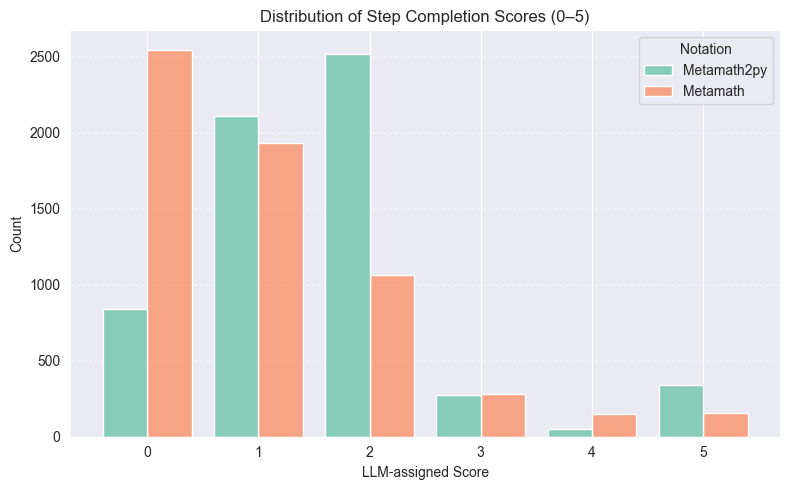
\includegraphics[scale=0.5]{step_completion_score.png}
  \caption{LLM-as-a-judge step completion scores.}
  \label{fig:fig1}
\end{figure}

Figure \ref{fig:fig1} shows the distribution of LLM-assigned scores (ranging from 0 to 5, where 5 is better)
evaluating
the
quality of
predicted next proof steps. Python-based representations demonstrate significantly better results compared to the original notation. Most Metamath-based completions received low scores (0 or 1), indicating the model's difficulty in interpreting symbolic notation without additional structural cues. In contrast, Python proofs exhibit a more balanced distribution, peaking at score 2 and with a noticeable portion receiving high scores (3–5).


\begin{figure}[H]
  \centering
  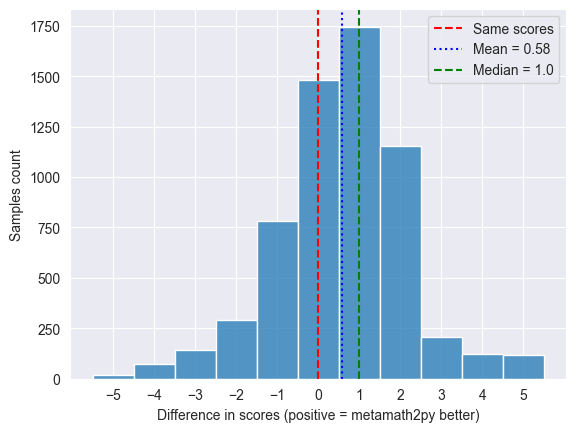
\includegraphics[scale=0.5]{scores_diff.png}
  \caption{Histogram of LLM-assigned score differences.}
  \label{fig:fig2}
\end{figure}


It is useful to compare the change in scores for each proof when the notation changes. Figure \ref{fig:fig2} shows
histogram of
LLM-assigned score differences between the Python-style proofs (metamath2py) and the
original notation. Positive values indicate samples where Metamath2py received higher scores. The
distribution is slightly skewed toward positive values, with a mean of 0.58 and median of 1.0, suggesting improved
step completion quality. The red dashed line marks equal scores; blue and green lines indicate
the mean and median difference, respectively.


This supports the hypothesis that translating formal proofs into a structured and more familiar format—such as Python code—makes it easier for language models to reason about them. Even without specialized adaptation to the task or notation, LLMs are more successful at generating the next proof step when working with representations aligned with their training distribution.




\section{Conclusion and Further Work}
\hspace{\parindent}
Our work aims to make the high-quality formal content of Metamath more accessible for use with modern large language models. By creating the Metamath2Py dataset, we preserve the rigor of proof verification while translating theorem statements and proofs into a format better suited for pretraining, finetuning, and other machine learning applications.

Future plans include leveraging this dataset to assist human theorem provers as well as  
developing fully automated theorem proving-covering the entire pipeline from natural language theorem
formulation to formal proof writing in a system like Metamath.  

The results of our work will be published as a dataset on Hugging Face (\href{https://huggingface.co/datasets/kamushekp/Metamath2Py}{link}) and as open-source code on GitHub (\href{https://github.com/kamushekp/metamath2py}{link}), both
under the MIT license.

\section{Acknowledgments}
\hspace{\parindent}
The author thanks Ph.D. Anton Konygin (konygin@imm.uran.ru), Scientific Researcher at the Krasovskii Institute of Mathematics and Mechanics, for valuable comments during the review process.




%Bibliography
\bibliographystyle{plain}
\bibliography{references}

\end{document}
